\abstract{These release notes describe the up-to-date features of
  PlanetMath's software system, Planetary.  The notes can be browsed
  online at \url{http://planetmath.org/planetaryreleasenotes}}

Figures \ref{ReaderView}, \ref{ProblemOne}, \ref{SolutionCareOfRay},
\ref{ProblemInCollection}, \ref{AttachableContent},
\ref{QuestionsPartI}, \ref{QuestionsPartII}, \ref{QuestionsPartIII},
\ref{BuddyListToCreate}, 
% \ref{BuddyListCreated},
% \ref{BuddyListViewed}, 
and \ref{TeamWorkflow}
%, \ref{InterlinkModule},
%\ref{ImageBacklinks},
% and \ref{MSCBrowsing}
show some of the key features of the Planetary system. The images are from the live system on \url{http://planetmath.org}. Footnotes provide more details on our implementation strategy and future plans.

\FloatBarrier

\begin{vplace}[0.7]
\begin{figure}[h]
\begin{center}
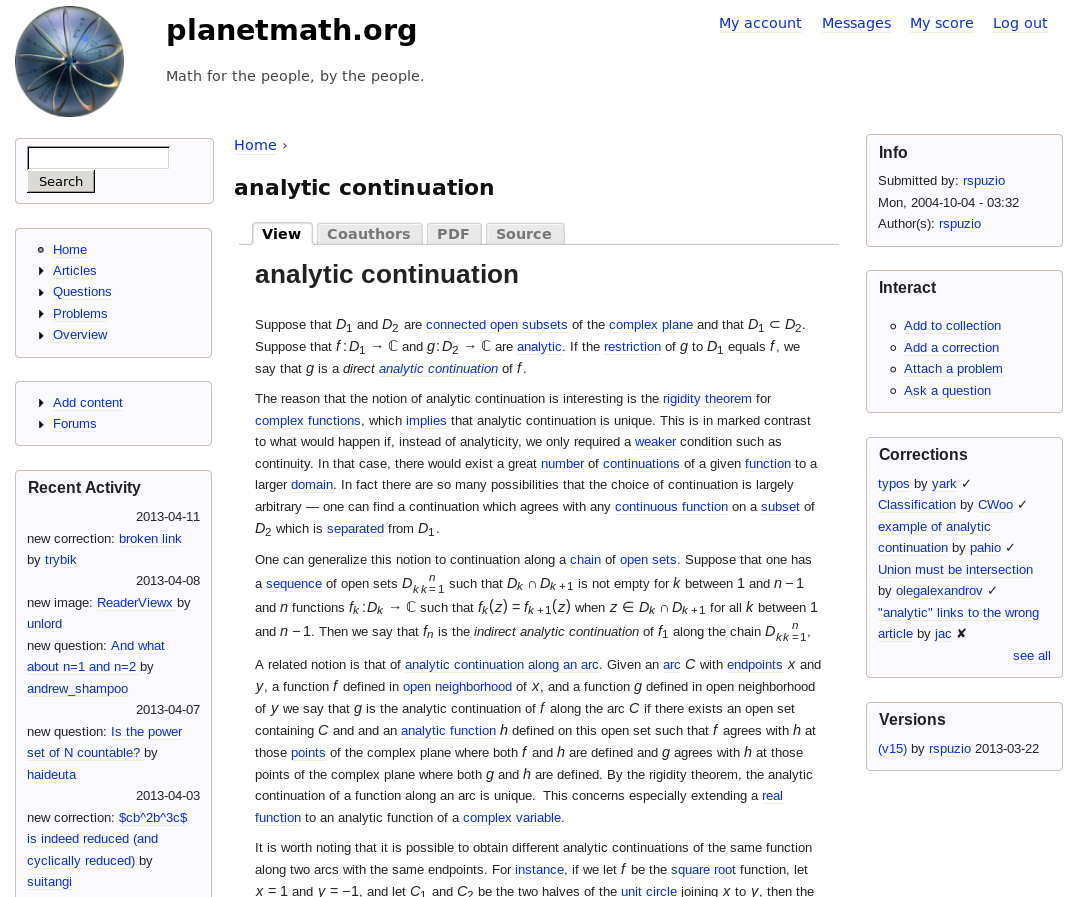
\includegraphics[width=.85\textwidth]{./inputs/ReaderView.png}
\end{center}
\caption{``Article UI'' (reader view), including problems attached to
  articles, with any metadata. \label{ReaderView}}
\end{figure}
\bigskip

Figure \ref{ReaderView} illustrates a key new feature of the system:
a block containing problems now shows up whenever the article has
attached problems.  The figure also illustrates interactions that are
available to any logged-in reader when browsing an encyclopedia
article, including adding a new problem, adding a correction, asking a
question, or adding the article to a collection.\footnote{The pattern
  for adding new localized interactions is exhibited in the {\sfdefault
    collection}, {\sfdefault problem}, etc., modules; and the ``Interact''
  block itself is managed in the {\sfdefault planetmath\_authorlinks}
  module. Thus, for instance, if we would like to be able to quickly
  attach articles --
  \url{https://github.com/KWARC/planetary/issues/342} -- or images
  \url{https://github.com/KWARC/planetary/issues/205} -- it will be a
  minor change.  Integrating JOBAD would provide a set of finer-grained
  reader-level interactions.}

\end{vplace}

\FloatBarrier

\begin{vplace}[0.7]
\begin{figure}[h]
\begin{center}
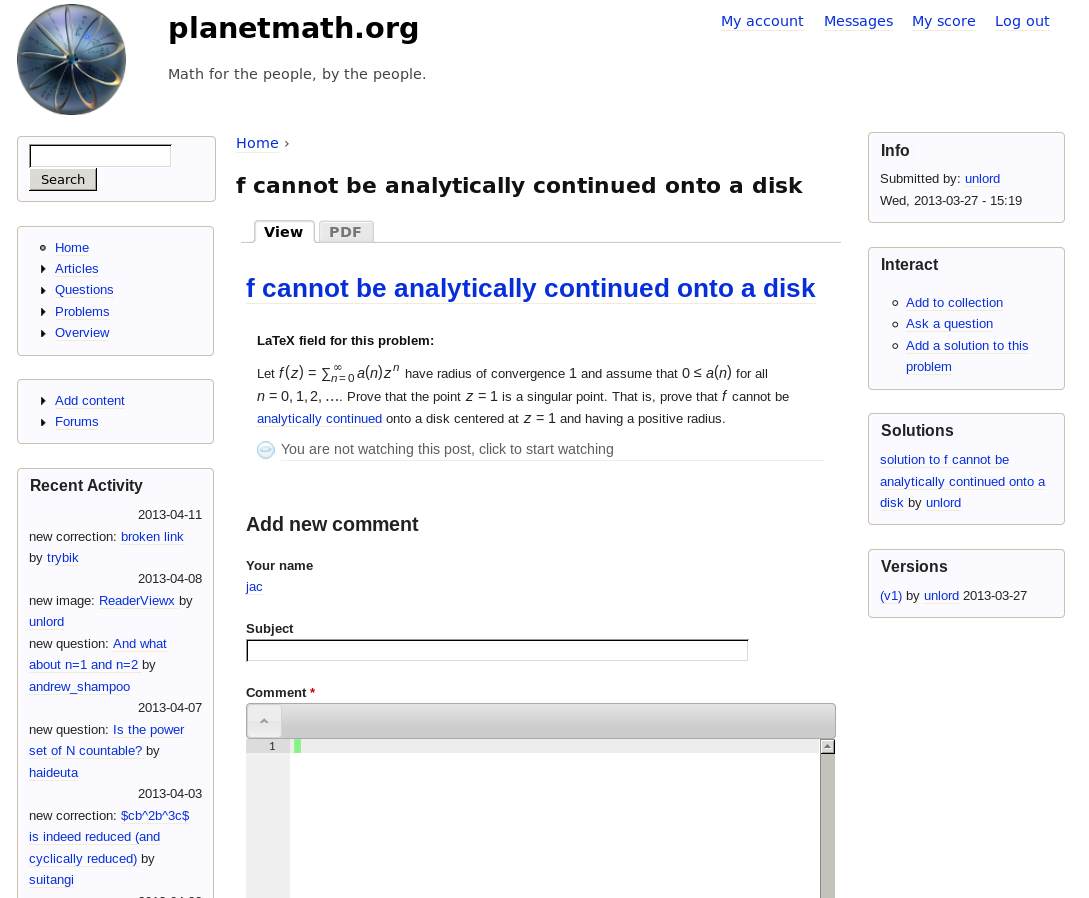
\includegraphics[width=.85\textwidth]{./inputs/ProblemOne.png}
\end{center}
\caption{Solutions attached to problems \label{ProblemOne}}
\end{figure}
\bigskip

Figure \ref{ProblemOne} shows a problem, with its own set of
interactions, including the ability to create a new solution.
Problems come with a ``Related Articles'' block that shows all
articles to which the problem has been attached.  Once solutions have
been added, they will be listed in another block.\footnote{Some users
  might prefer \emph{not} to know that solutions are available until
  they specifically ask for a hint.  We'll work to accommodate this
  preference, see \url{https://github.com/KWARC/planetary/issues/343}}
\end{vplace}

\newpage
\FloatBarrier

\begin{vplace}[0.7]
\begin{figure}[h]
\begin{center}
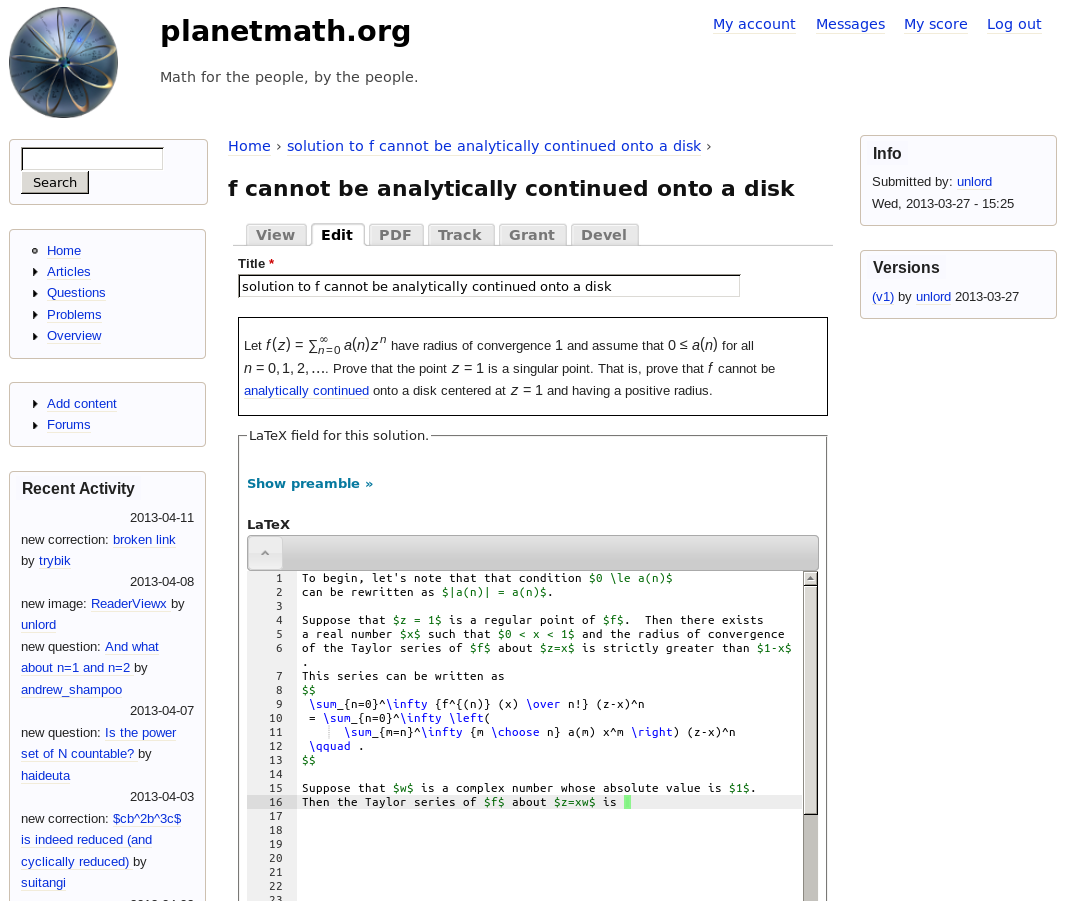
\includegraphics[width=.85\textwidth]{./inputs/SolutionCareOfRay.png}
\end{center}
\caption{Solving a problem \label{SolutionCareOfRay}}
\end{figure}
\bigskip

Figure \ref{SolutionCareOfRay} shows the new \LaTeX\ editor, with the
user in the process of adding a solution to the problem we just looked
at.  The text of the problem statement is copied onto the screen above
the \LaTeX\ field, so the user doesn't have to open multiple tabs to
keep track of the basic information they need to solve the
problem.\footnote{\label{fn:course-packet}In fact, we could do much
  better, by generating a ``course packet'' on the fly for any
  problem, and having this available to the user when they are working
  on a problem: \url{https://github.com/KWARC/planetary/issues/323}.
  Feedback on the quality of automatically retrieved content could be
  used to feed improve the quality of the corpus metadata, and
  potentially the autolinking algorithm itself.}
\end{vplace}

\newpage
\FloatBarrier

\begin{vplace}[0.7]
\begin{figure}[h]
\begin{center}
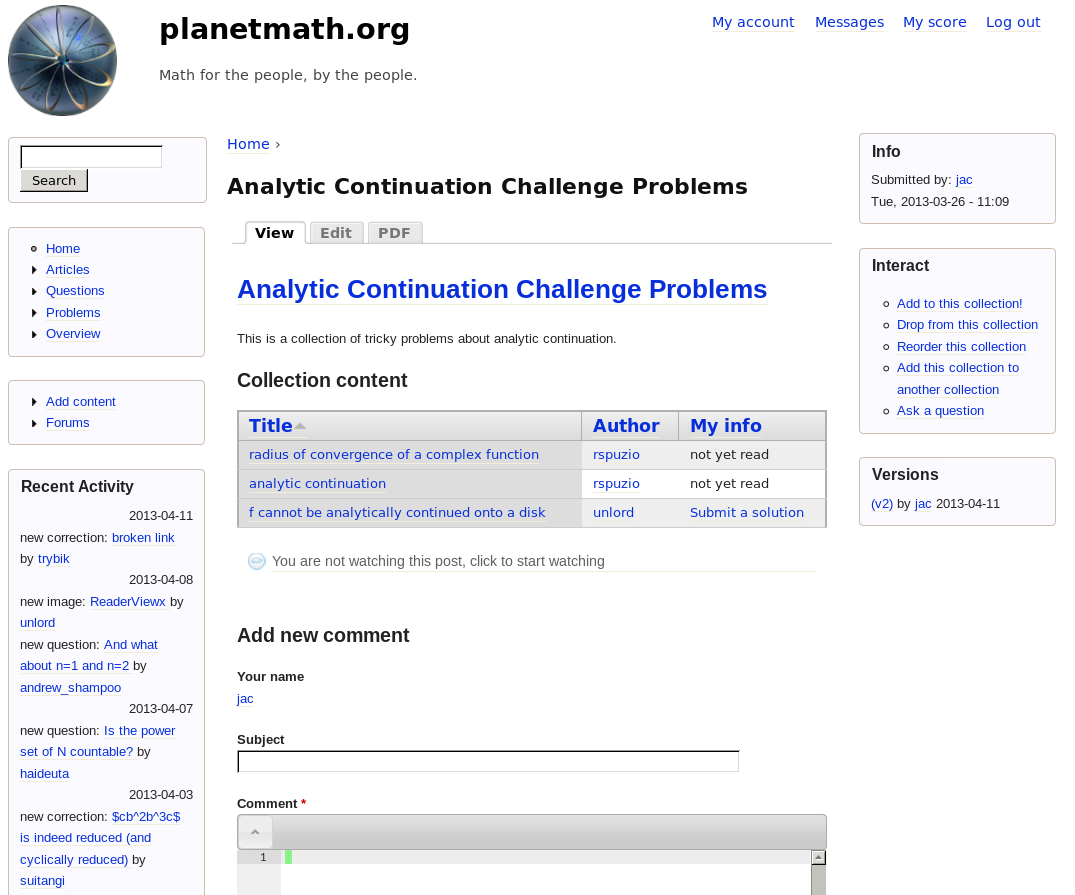
\includegraphics[width=.85\textwidth]{./inputs/ProblemInCollection.png}
\end{center}
\caption{Paradata that shows up as a user works their way through a collection \label{ProblemInCollection}}
\end{figure}
\bigskip

Articles, problems, and other content can be added to collections,
which function as ``playlists'' for math content, as illustrated in
Figure \ref{ProblemInCollection}.  As the user works their way through
the problems in a given collection, personalized metadata (or, more
precisely, \emph{paradata}) shows up in the ``My info'' field.  If
another user adds a review for a solution, this information will
appear.  Although collections are just ordered lists, they can also
contain other collections, allowing the user to create and share a
tree-like outline, or more general network structure of paths through
the content.
\end{vplace}

\newpage
\FloatBarrier

\begin{vplace}[0.7]
\begin{figure}[h]
\begin{center}
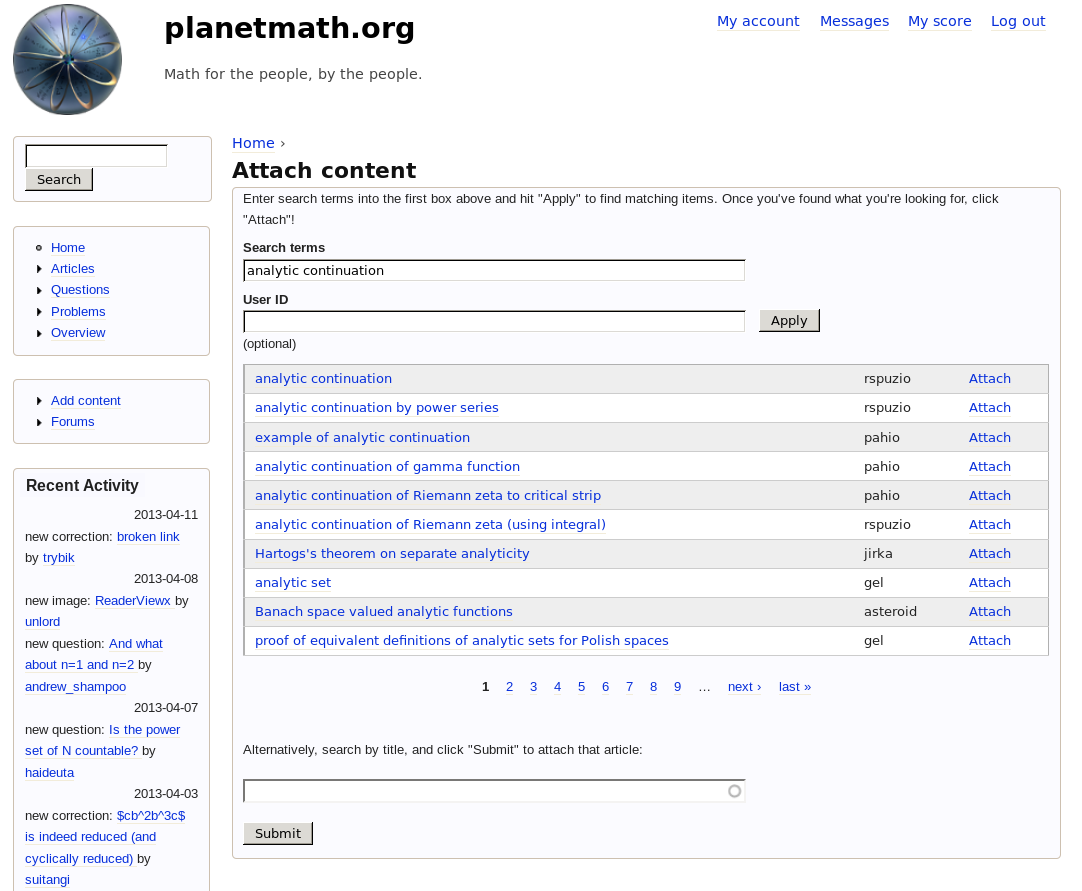
\includegraphics[width=.85\textwidth]{./inputs/AttachableContent.png}
\end{center}
\caption{Search being used to add items to a collection \label{AttachableContent}}
\end{figure}
\bigskip

Figure \ref{AttachableContent} shows a common UI that is used with
collections, groups, and questions.  Here, the user is adding an item
to a collection using free-text search.  New member objects can also
be added by autocompleting on the title, if the title is known, or
added directly.
\end{vplace}

\newpage
\FloatBarrier

\begin{vplace}[0.7]
\begin{figure}[h]
\begin{center}
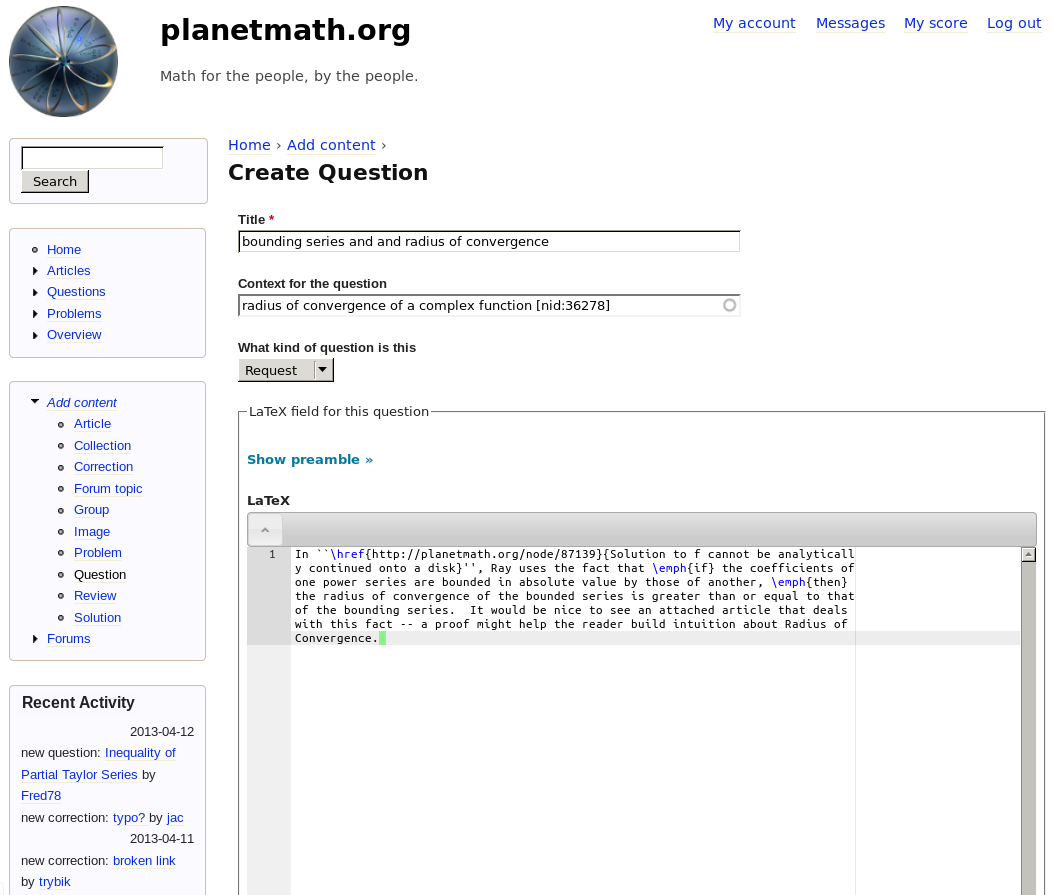
\includegraphics[width=.85\textwidth]{./inputs/QuestionsPartI.png}
\end{center}
\caption{Adding a question \label{QuestionsPartI}}
\end{figure}
\bigskip

Figure \ref{QuestionsPartI} shows a question being added ``in
context'' -- which would have been done using the ``Ask a question''
UI element, like as pictured in Figure \ref{ReaderView}.  Currently,
articles, problems, collections, and solutions can have questions
attached to them about them.  The user can also ask a question without
specifying the context by using the ``Add content'' menu item from the
left sidebar directly.  
\end{vplace}

\newpage
\FloatBarrier

\begin{vplace}[0.7]
\begin{figure}[h]
\begin{center}
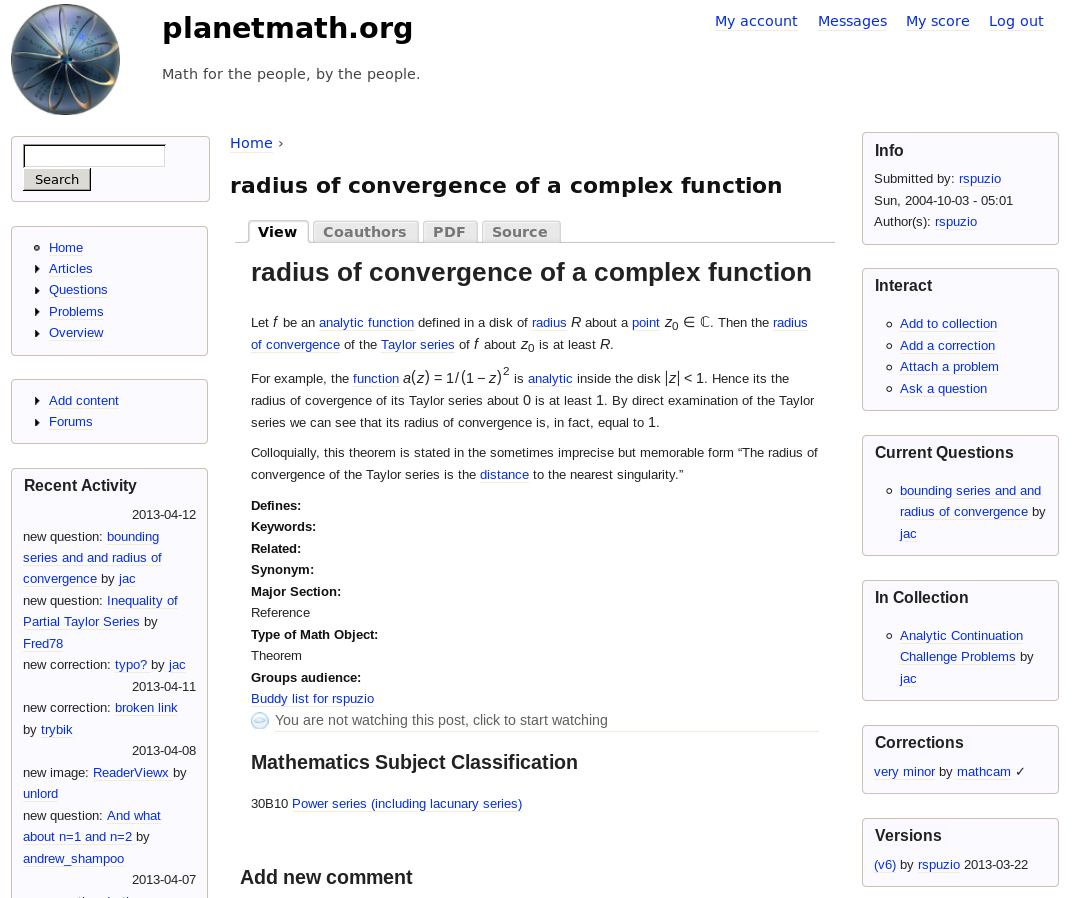
\includegraphics[width=.85\textwidth]{./inputs/QuestionsPartII.png}
\end{center}
\caption{Current questions appear in context \label{QuestionsPartII}}
\end{figure}
\bigskip

If a question was asked ``in context'', a link to the question shows
up in the relevant context, as depicted in Figure
\ref{QuestionsPartII}.  Questions also show up in the left-hand
sidebar along with other recent activity, and this is persisted across
the site.  This is a essentially a sort of light-weight free
advertising for users who contribute questions.

Questions also show up in a special-purpose
feed.\footnote{\url{http://planetmath.org/questions}} Note that with
these features, we are \emph{not} trying to clone the interactions on
StackExchange, although we are certainly inspired by the activities
there.  Rather, we are working to use questions and other new features
together with the encyclopedia, to help build a cohesive and coherent
mathematical knowledge base.
\end{vplace}

\newpage
\FloatBarrier

\begin{vplace}[0.7]
\begin{figure}[h]
\begin{center}
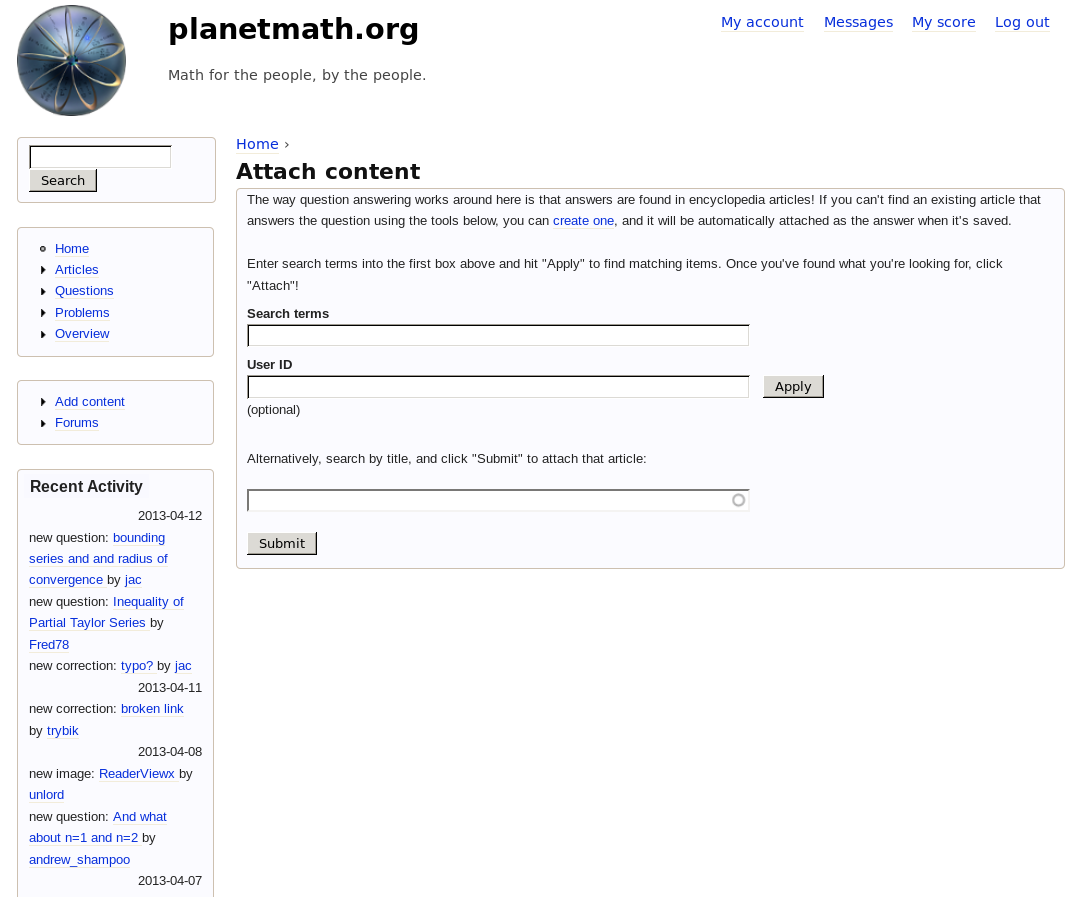
\includegraphics[width=.85\textwidth]{./inputs/QuestionsPartIII.png}
\end{center}
\caption{Making improvements to the encyclopedia when answering a question \label{QuestionsPartIII}}
\end{figure}
\bigskip

As indicated in Figure \ref{QuestionsPartIII} answers are supposed to
appear in encyclopedia articles.  That means the answerer can either
point to an existing article (and add a brief ``memorandum'') -- or
add a new article.  This way, questions that deal with topics that
aren't adequately covered by current articles should lead to
improvements to the encyclopedia.\footnote{Data coming from questions
  together with other aspects of the domain model and user models
  should eventually be quite useful for making recommendations.  We
  currently at a more preliminary stage, providing the models we can
  use to understand the sorts of recommendations that could be
  useful.}
\end{vplace}

\newpage
\FloatBarrier

\begin{vplace}[0.7]
\begin{figure}[h]
\begin{center}
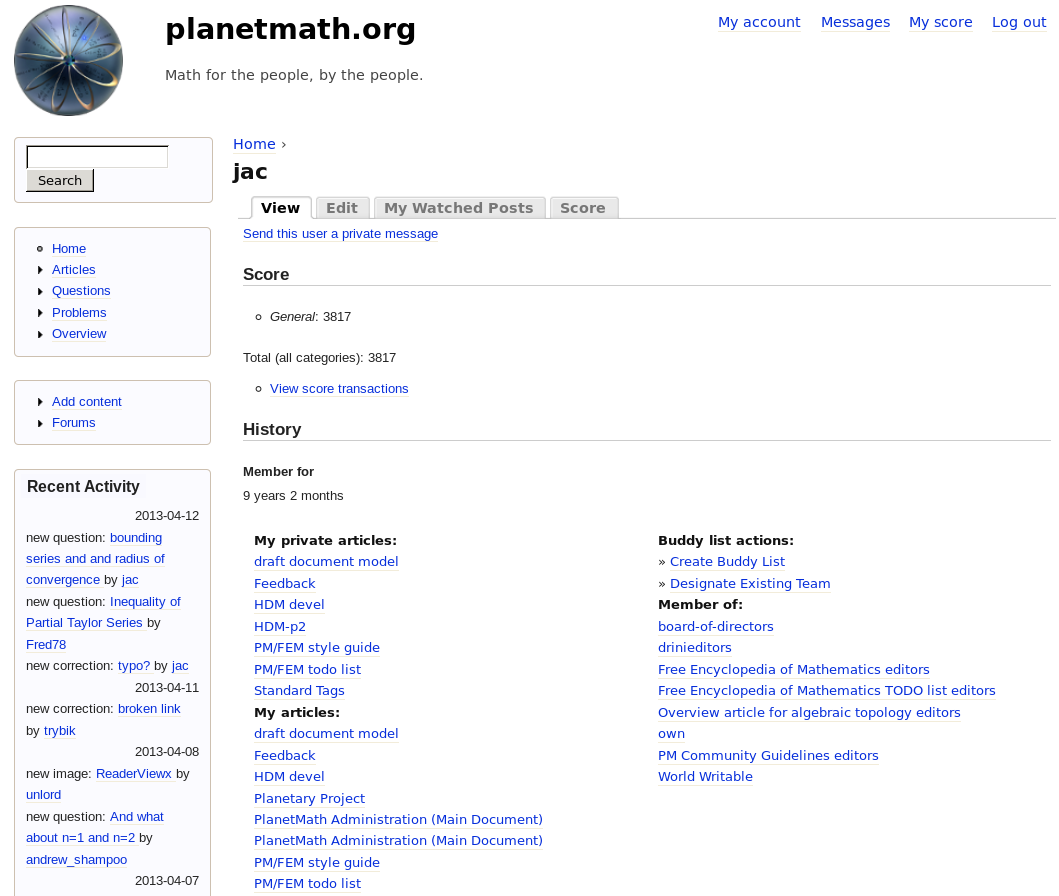
\includegraphics[width=.85\textwidth]{./inputs/BuddyListToCreate.png}
\end{center}
\caption{Groups workflow: the option to create a buddy list \label{BuddyListToCreate}}
\end{figure}
\bigskip

Figure \ref{BuddyListToCreate} illustrates one of the new, simple
mechanisms that Planetary provides for managing access to articles.
The user can create a ``buddy list'' and everyone on the list will
have access to all of his or her articles.  An existing team can also
be specified, in which case, all members of that team will have access
to each of the user's articles.  In particular, if a user wants to
make all of their articles world editable, they can simply specify the
World Writeable team as their buddy list.
\end{vplace}

\newpage
\FloatBarrier

\begin{vplace}[0.7]
\begin{figure}[h]
\begin{center}
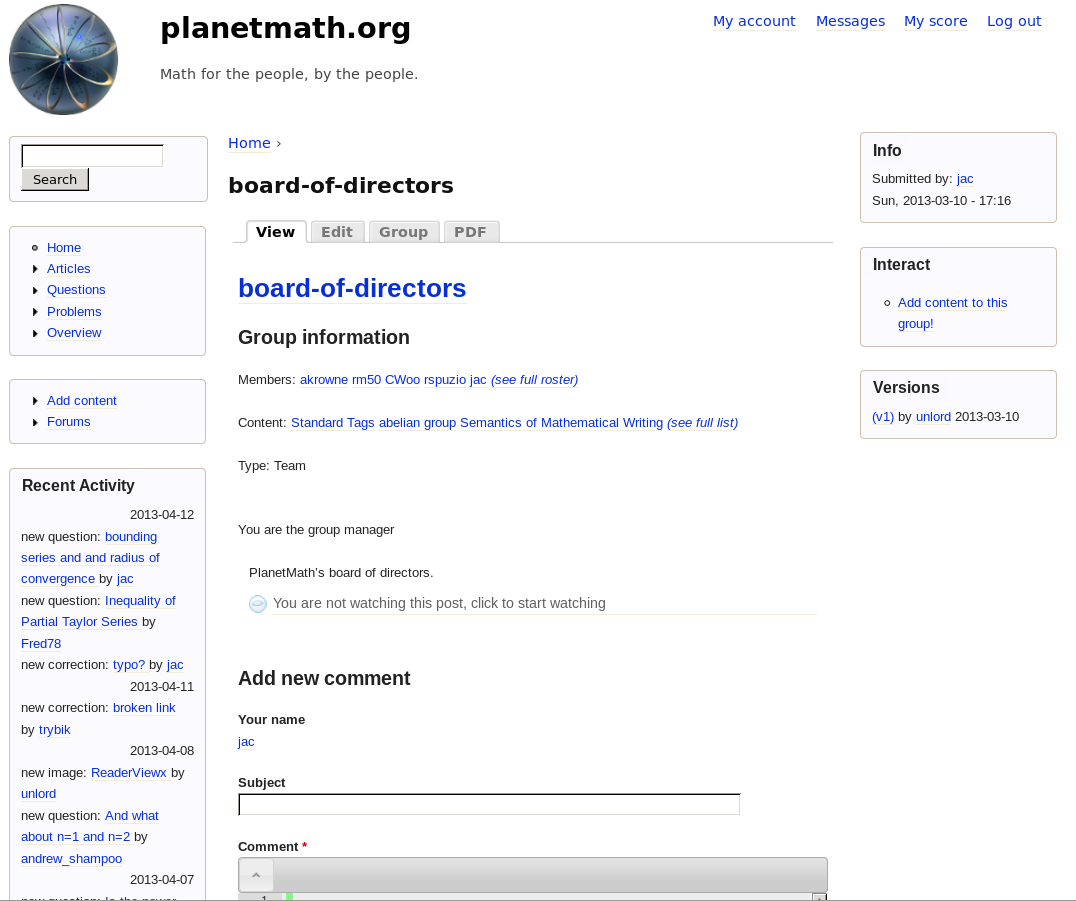
\includegraphics[width=.85\textwidth]{./inputs/TeamWorkflow.png}
\end{center}
\caption{Groups workflow: a team's shared content \label{TeamWorkflow}}
\end{figure}
\bigskip

Teams (Figure \ref{TeamWorkflow}) are similar to buddy lists.  Any
content that is added to a team is made editable by all of that team's
members -- but accordingly, group content can only be shared by
someone who already has editing permissions.  Collections can be used
to assemble content that are is not editable to others -- or indeed to
the collection-maker.\footnote{Note that being able to edit an article
  does not automatically make you a ``coauthor'', although your
  username will be stored in the article's revision history.  This
  allows trusted members of a buddy list or team to make small
  corrections, without necessarily assuming full author status.}
\end{vplace}

\FloatBarrier
